\chapter{IEEE}
\label{chapterlabel3}


\section{Introduction}

INSERT is the world's first clinical simultaneous SPECT/MRI system. The system is a brain SPECT insert, designed for complete integration with any clinical MRI system. The stationary insert system is composed of a partial ring of 20 detector units, each with a 10x5 $cm^2$ CsI(TI) crystal, silicon photomultiplier (SiPM) and ASIC readout. A novel MR compatible collimator; the multi-mini-slit-slat (MSS), \cite{7430894}, was designed specifically for the compatibility and clinical needs of the system. The use of the MSS collimator requires the implementation of a specific calibration procedure, which was established on a single detector system, \cite{8340862}, and initially tested on a semi-operational system, \cite{inproceedings}.

The partial ring MSS collimator imposes some limitations on the system's sampling. In this work we utilise a dual reconstruction technique in order to improve angular sampling of the system. Due to hardware issues we had cases of detection failure in which data were missing across a few affected units. The calibration and event reconstruction techniques were found to provide a means of correcting missing event data. The limitations of the prototype were overcome by the calibration procedure, producing successful reconstructed phantom images, which were further improved by the dual acquisition protocol.   

\section{Methods}

\subsection{Event Reconstruction}
The system carries out event reconstruction with a maximum likelihood (ML) algorithm. The ML reconstruction requires modelling of each SiPM Light Response Function (LRF). LRF models were constructed for each detector channel, derived from a uniformity flood acquisition, \cite{6359814}. LRF modelling has previously been used to evaluate the detectors, \cite{8069405}; here we establish use of the models as a correction for hardware failure. The LRF is able to account for missing event data in a given channel by modelling the known spatial response and interpolating counts from surrounding channels. This methods is limited to small regions as it cannot correct large areas of missing data. 


\subsection{System Calibration}
 The calibration procedure involves two steps; detector calibration and system calibration. The detector calibration involved standard linearity and uniformity corrections of the projection data. The linearity and uniformity corrections were carried out with simple transformations of the projection data using a flood source and linearity collimators. The system calibration consists of a geometric and sensitivity calibration followed by event re-sampling; this procedure accounts for the MSS system design. 
 
The geometric calibration has been established previously, \cite{8340862}. The sensitivity calibration required data with a planar phantom, filled with 50 MBq of $^{99m}Tc$ solution, and placed close to each of the collimated detectors. The sensitivity profiles were fitted using equation (\ref{sens_model}), where $\phi$ is the sampling angle, $G_{σ}(\phi)$ is a Gaussian function and the summation is done over all mini-slits $i$ for each collimator section $j$. Fig. \ref{fig_sensprof} shows examples of sensitivity profiles for two different collimator sections and the corresponding fits.

\begin{equation}
%\vspace{-0.2cm}
\label{sens_model}
S_{j}(\phi) = \sum_{i} G_{\sigma}(\phi) \ast A_{i,j} \cos^{p}{\phi} + b_{j}(\phi)
%\vspace{-0.2cm}
\end{equation}

The final step in the calibration involves re-sampling the projection data to produce projection reconstructions in object domain. Accounting for the system geometry, the radial position of each event is calculated. The events are then re-ordered with respect to the radial position from the centre of the FOV. The result allows for easier visual analysis of the acquired data; at this stage the data are completely corrected and ready for reconstruction. 

\begin{figure}[!t]
%\vspace{-0.2cm}
\centering
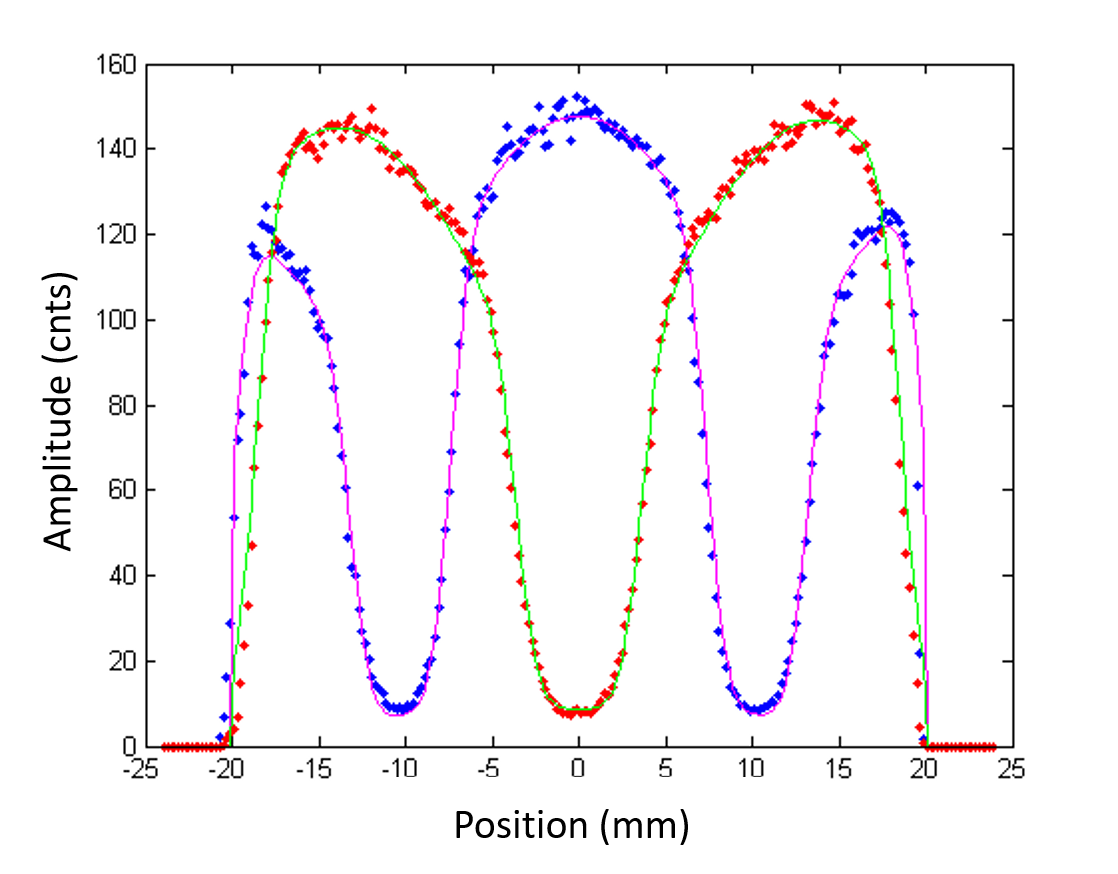
\includegraphics[width=2.9in]{figures/sns_prof.png}

\caption{Sensitivity profiles for two collimator sections and fitted analytical functions.}
\label{fig_sensprof}
%\vspace{-0.2cm}
\end{figure}
 
\subsection{Image Reconstruction}

The calibration corrected data are reconstructed using Maximum Likelihood Estimation Maximisation (ML-EM), \cite{4307558} in combination with angular blurring, \cite{bousse2013angular}; figure \ref{fig_ImageRes} shows capillary phantom reconstructed in this way. The image shows promising results across the field-of-view (FOV) however the reconstruction is limited by the angular sampling of the MSS collimator and the partial ring system. We were able to overcome this by introducing a dual reconstruction of two sets of acquisition data. As an additional option, the phantom data may be acquired at two angular positions, separated by a rotation about the z-axis. The second acquisition will provide projections from the missing region of the detector ring; an offset of half a detector also provides data in between each unit and provides improved angular sampling. The increase sampling overcomes detection failure over a large area; if a large region is missing, the rotated position is able to capture events from another detector unit. 

The known positions of each acquisition are treated as two subsets, reconstructing both sets of data simultaneously, analogous to an ordered subset expectation maximisation (OSEM) algorithm, \cite{363108}. The images were further improved with the use of structural information, simulating the use of MRI in the system. A post reconstruction partial volume correction (PVC) was carried out on the dual reconstructed images, \cite{Erlandsson_2012}.


\section{Results}
 The reconstructed capillary phantom images were used to determine the system image resolution. The trans-axial resolution was determined at various radial positions across the detector's 20x20x9 $cm^3$ FOV, Fig. \ref{fig_resolution}. Measurements of the radial and tangential resolution show the effects of partial ring reconstruction; the bottom capillaries in Fig. \ref{fig_ImageRes} are in the region with no detectors and so the reconstructed values have a greater error. The system resolution is most stable closer to the centre of the FOV where the partial ring effects are less prominent. The standard deviation in resolution is greatest on the edge of the FOV where the point sources appear to stretch radially, Table \ref{table_reso}.
 
 The phantom acquisitions include a Cold Rods phantom, a Hot Spheres phantoms and a 2D Hoffman Brain phantom. Figures, \ref{fig_cold}, \ref{fig_Hot} and \ref{fig_Hoffman}, show the results of the dual reconstruction method and the improvement from the post reconstruction PVC. 



\begin{table}[!b]
% increase table row spacing, adjust to taste
\renewcommand{\arraystretch}{1.3}

\captionsetup{font=small}
\caption{Trans-axial Resolution}
\label{table_reso}
\centering

\begin{tabular}{|p{2.5cm}|p{2.8cm}|p{2.8cm}|}
\hline
Radial Position [mm]& Mean Radial Resolution [mm]& Mean Tangential Resolution [mm] \\
\hline
 25 & 9.39 $\pm$ 0.66 & 7.95 $\pm$ 0.51\\
\hline
 50 & 8.87 $\pm$ 1.15 & 7.31 $\pm$ 0.25\\
\hline
 75 & 9.49 $\pm$ 1.27 & 6.59 $\pm$ 0.95\\
\hline
 100 & 8.83 $\pm$ 2.00 & 5.1629 $\pm$ 1.08\\
\hline
\end{tabular}
\end{table}



\begin{figure}[!t]
%\vspace{-0.2cm}
\centering
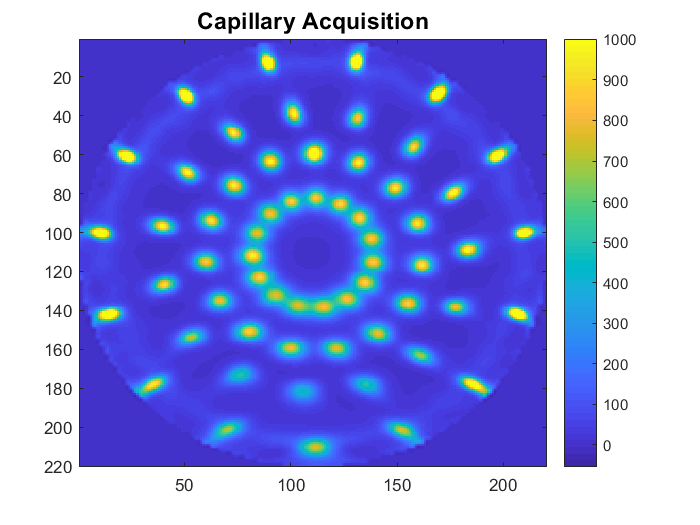
\includegraphics[width=3in]{figures/Capillary_newLRF.PNG}

\caption{The reconstructed capillary phantoms after corrections. The capillaries had 1mm diameter; each were filled with 10 MBq of $^{99m}Tc$ and were scanned for 5 minutes.}
\label{fig_ImageRes}
%\vspace{-0.2cm}
\end{figure}

\begin{figure}[!t]
%\vspace{-0.2cm}
\centering
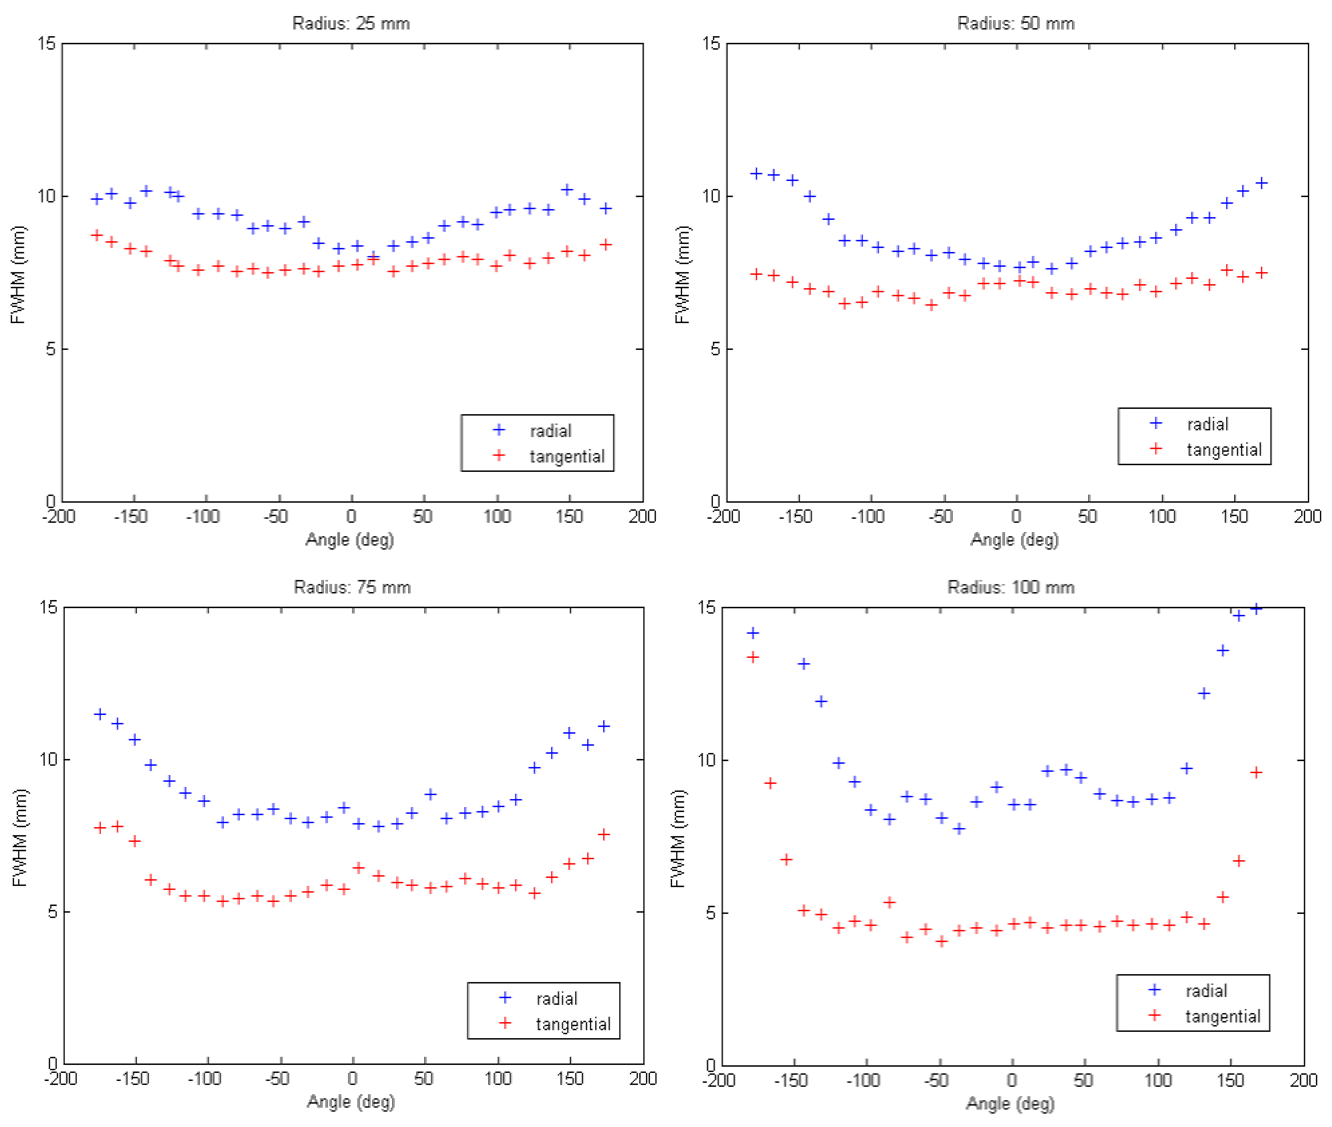
\includegraphics[width=3.4in]{figures/resolutions.png}

\caption{Resolution of capillaries at 4 radial positions against the angular position in the FOV.}
\label{fig_resolution}
%\vspace{-0.2cm}
\end{figure}

\begin{figure}[!t]
%\vspace{-0.2cm}
\centering
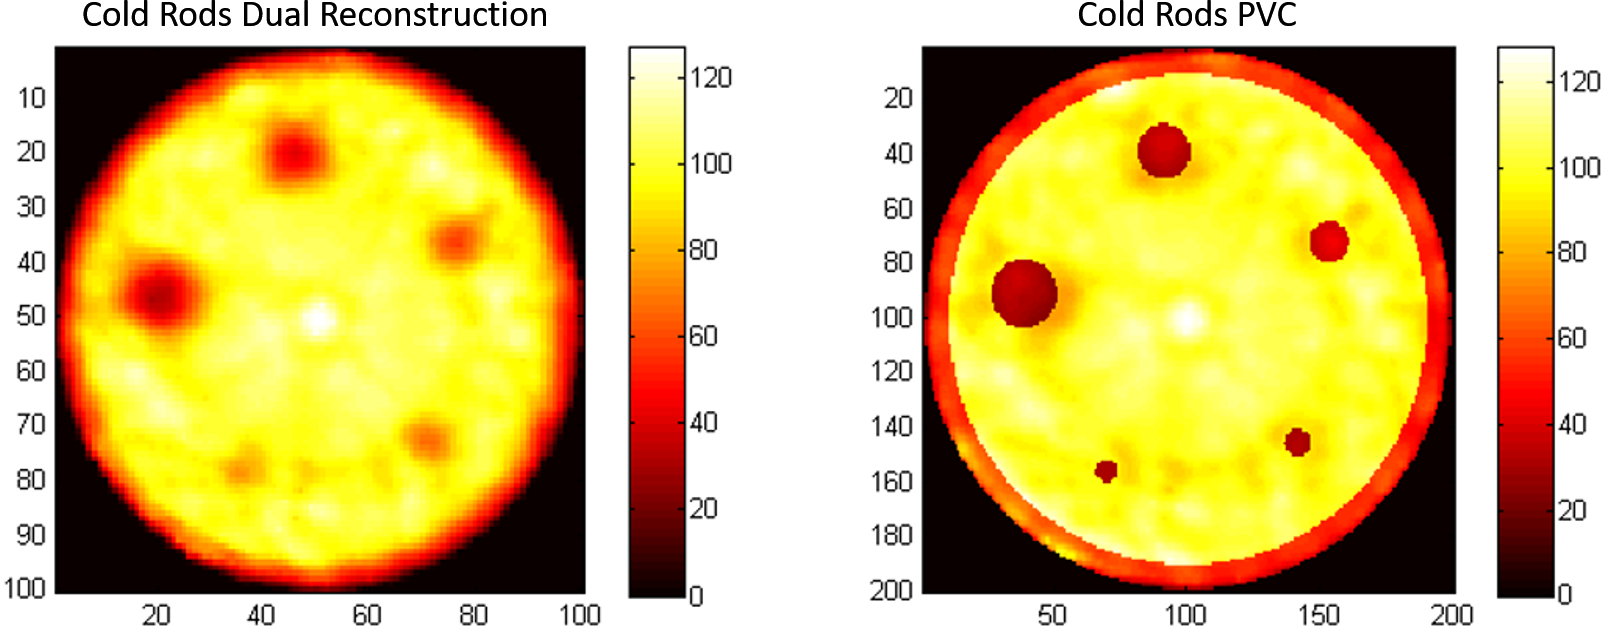
\includegraphics[width=3.5in]{figures/ColdRods.png}

\caption{Cylinder phantom of 50 MBq of activity and cold rods of diameters; 8, 10, 15, 20 and 25 mm.}
\label{fig_cold}
%\vspace{-0.2cm}
\end{figure}

\begin{figure}[!t]
%\vspace{-0.2cm}
\centering
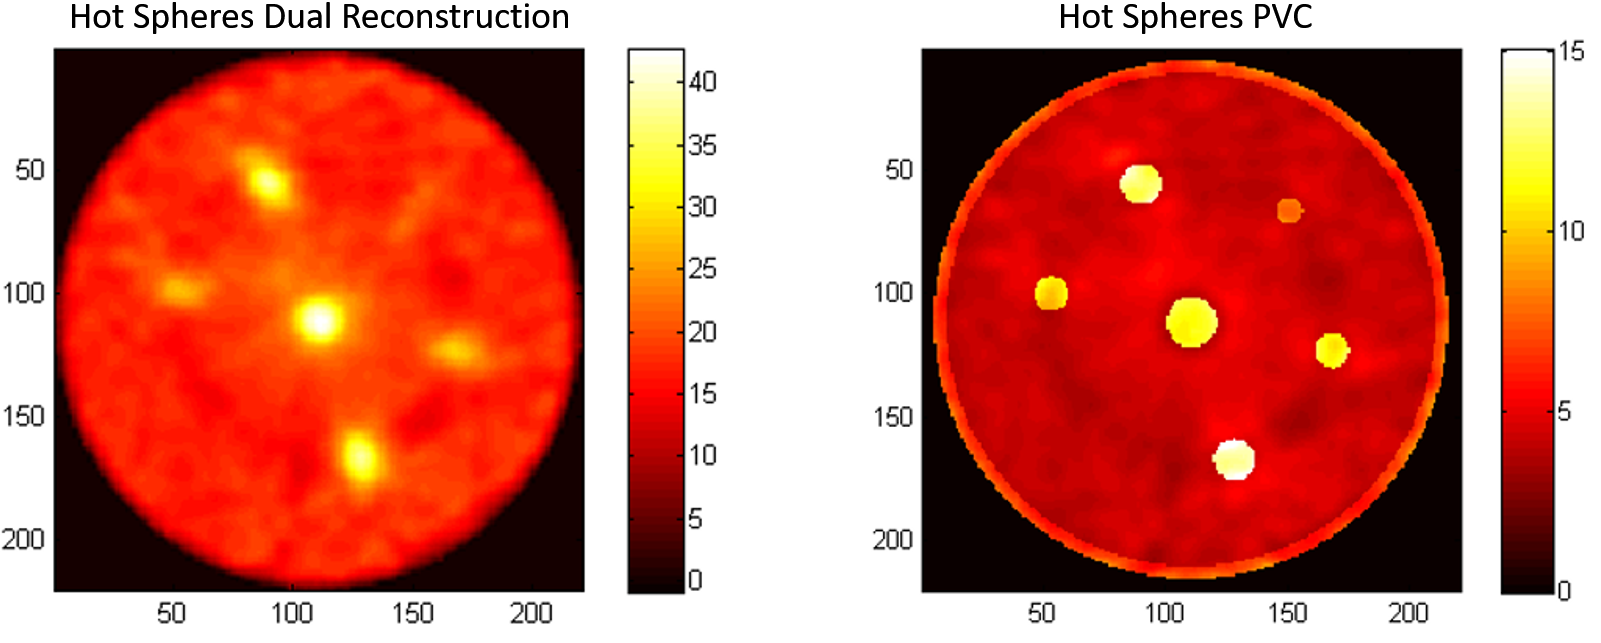
\includegraphics[width=3.5in]{figures/HotSpheres.png}

\caption{60 MBq to a ratio of 8:1 in the hot spheres of diameters; 11, 14, 17, 21 mm.}
\label{fig_Hot}
%\vspace{-0.2cm}
\end{figure}

\begin{figure}[!t]
%\vspace{-0.2cm}
\centering
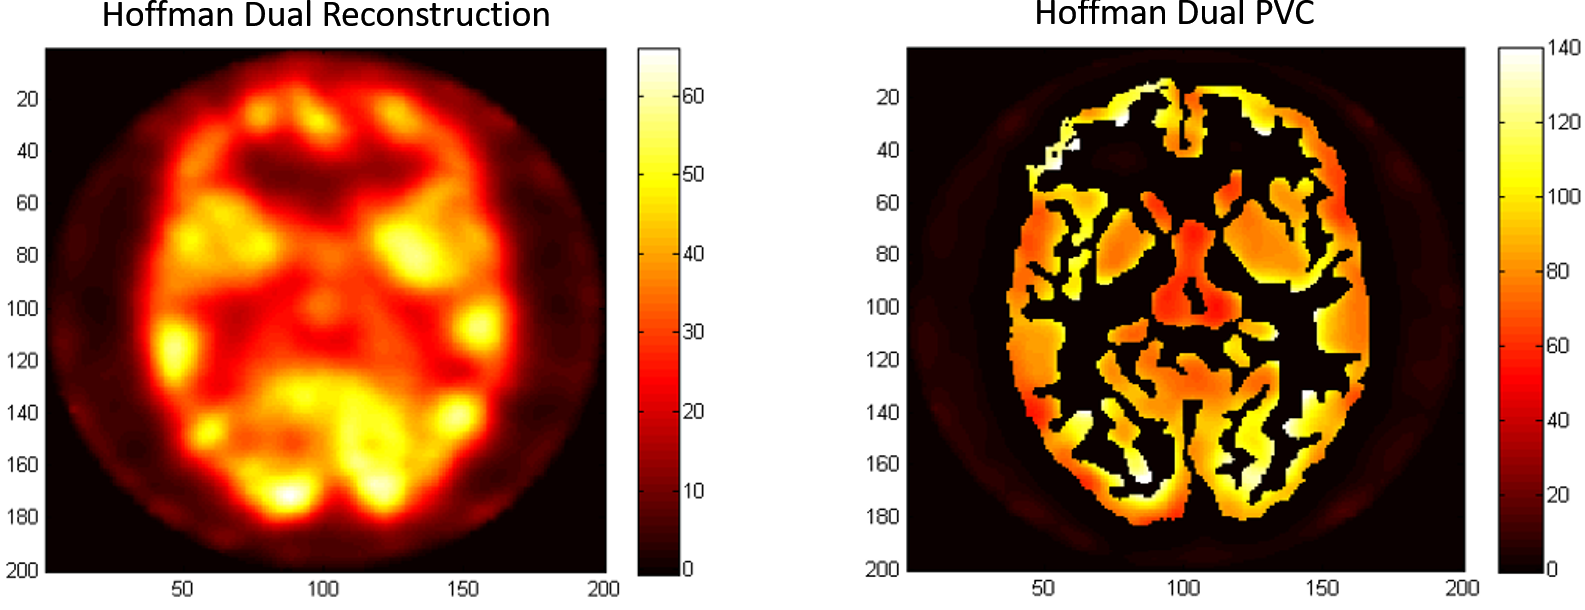
\includegraphics[width=3.5in]{figures/Hoffman.png}

\caption{2D Hoffman phantom with activity 25 MBq.}
\label{fig_Hoffman}
%\vspace{-0.2cm}
\end{figure}


\section{Conclusion and Discussion}
Overall the acquisition and reconstruction methods have demonstrated effective means of generating reconstructed images from incomplete data acquisition. We are able to correct for inhomogeneity in the detectors and produce correct projection data. The sensitivity model is able to improve image reconstruction by accounting for geometric variations across the projections. The results of this research improved the processing of INSERT projection data and introduced dual reconstruction, which can be used to benefit the system's clinical performance.
The images acquired show some limitation in the system, however we are able to produce good quality images from the SPECT system alone. Implementing the dual reconstruction has shown to improve the images, however we treat this as an extension to our system, the system is able to function and produce good quality images without this step. The INSERT detector technology has undergone preliminary characterisation of the SPECT system, \cite{8891783}, however complete MR compatibility has only been validated in the preclinical system, \cite{8612977}. Future work will set out to test the system in a clinical MR environment and to streamline calibration and acquisition procedures for routine use. The use of MR data will improve the images further and demonstrate the potential of the fully operational system.   

